% Created 2019-05-02 Thu 18:17
% Intended LaTeX compiler: pdflatex
\documentclass[11pt]{article}
\usepackage[utf8]{inputenc}
\usepackage[T1]{fontenc}
\usepackage{graphicx}
\usepackage{grffile}
\usepackage{longtable}
\usepackage{wrapfig}
\usepackage{rotating}
\usepackage[normalem]{ulem}
\usepackage{amsmath}
\usepackage{textcomp}
\usepackage{amssymb}
\usepackage{capt-of}
\usepackage{hyperref}
\usepackage[margin=0.5in]{geometry}
\author{Andrew Chen}
\date{\today}
\title{Deep Learning Final Notes}
\hypersetup{
 pdfauthor={Andrew Chen},
 pdftitle={Deep Learning Final Notes},
 pdfkeywords={},
 pdfsubject={},
 pdfcreator={Emacs 26.1 (Org mode 9.1.14)}, 
 pdflang={English}}
\begin{document}

\maketitle


\section{Machine Learning Basics}
\label{sec:orgf27ab05}

\subsection{Dimensionality Reduction}
\label{sec:orgc33b697}
\begin{itemize}
\item Supervised: Linear Discriminant Analysis
\item Unsupervised: PCA and Autoencoder
\end{itemize}

\section{CNN}
\label{sec:orgcfaeff9}

\subsection{Tricks to Know For Better Model Generalization}
\label{sec:org7f65c36}

\begin{enumerate}
\item Dropout
\begin{enumerate}
\item Works because it forces the model to make a decision with limited information, thereby eliminating a lot of unnecessary parameters
\end{enumerate}
\item Data Augmentation
\item Pre-train on different Larger Dataset
\item Ensemble methods
\begin{enumerate}
\item Have multiple models make a prediction and take the majority vote
\end{enumerate}
\item Multitask learning
\begin{enumerate}
\item Training a set of lower level layers and then later on training top level Conv layers for a specific task
\begin{enumerate}
\item ie: Train low level layers for learning low level features, and then train conv layers to recognize face, age, race, etc.
\end{enumerate}
\end{enumerate}
\end{enumerate}

\subsection{Tricks for Better Optimization}
\label{sec:org8e7236a}

\begin{enumerate}
\item Batch Normalization
\begin{enumerate}
\item Change the scale of the metrics which reduces condition number of matrix
\item Better conditioned Hessian -> Faster Convergence
\item Every feature has 0 mean and unit variance
\end{enumerate}
\item Gradient Injection
\item Skip Connections
\end{enumerate}

\section{Misc ML Facts}
\label{sec:orgbed4260}

\begin{enumerate}
\item In higher dimensions, it becomes improbable to find global minimum
\begin{enumerate}
\item You will find saddle points and local minima
\item If you use GD, you will probably find a Saddle point because gradient near saddle points is near 0
\item SGD can find local minima because it's random and noisy
\end{enumerate}
\item Large Batch Size -> poor generalization
\begin{enumerate}
\item Large Batch size -> faster training
\end{enumerate}
\end{enumerate}

\section{RNN}
\label{sec:org7618528}

\subsection{Basic Steps of Text Processing}
\label{sec:orged3d45f}

\begin{enumerate}
\item Tokenize corpus
\item Encode tokens
\item Align encodings by padding shorter encodings with 0s in the front
\item Convert encodings (vectors) to work embeddings (matrix)
\begin{enumerate}
\item Train to create a matrix of (vocab\_size x embedding dimension)
\item For each encoding (scalar), convert it to a vector, and the final result will be a matrix where each vector within represents a word (in vector form)
\end{enumerate}
\item Rules of Thumb
\begin{enumerate}
\item Always use LSTM over SimpleRNN
\item Always use LSTM dropout to alleviate overfitting
\item Use Bi-LSTM whenever possible
\item Use stacked LSTM if sample size is big
\item Pretrain the embedding layer if sample size is small
\end{enumerate}
\item SimpleRNN Implementation
\begin{figure}[htbp]
\centering
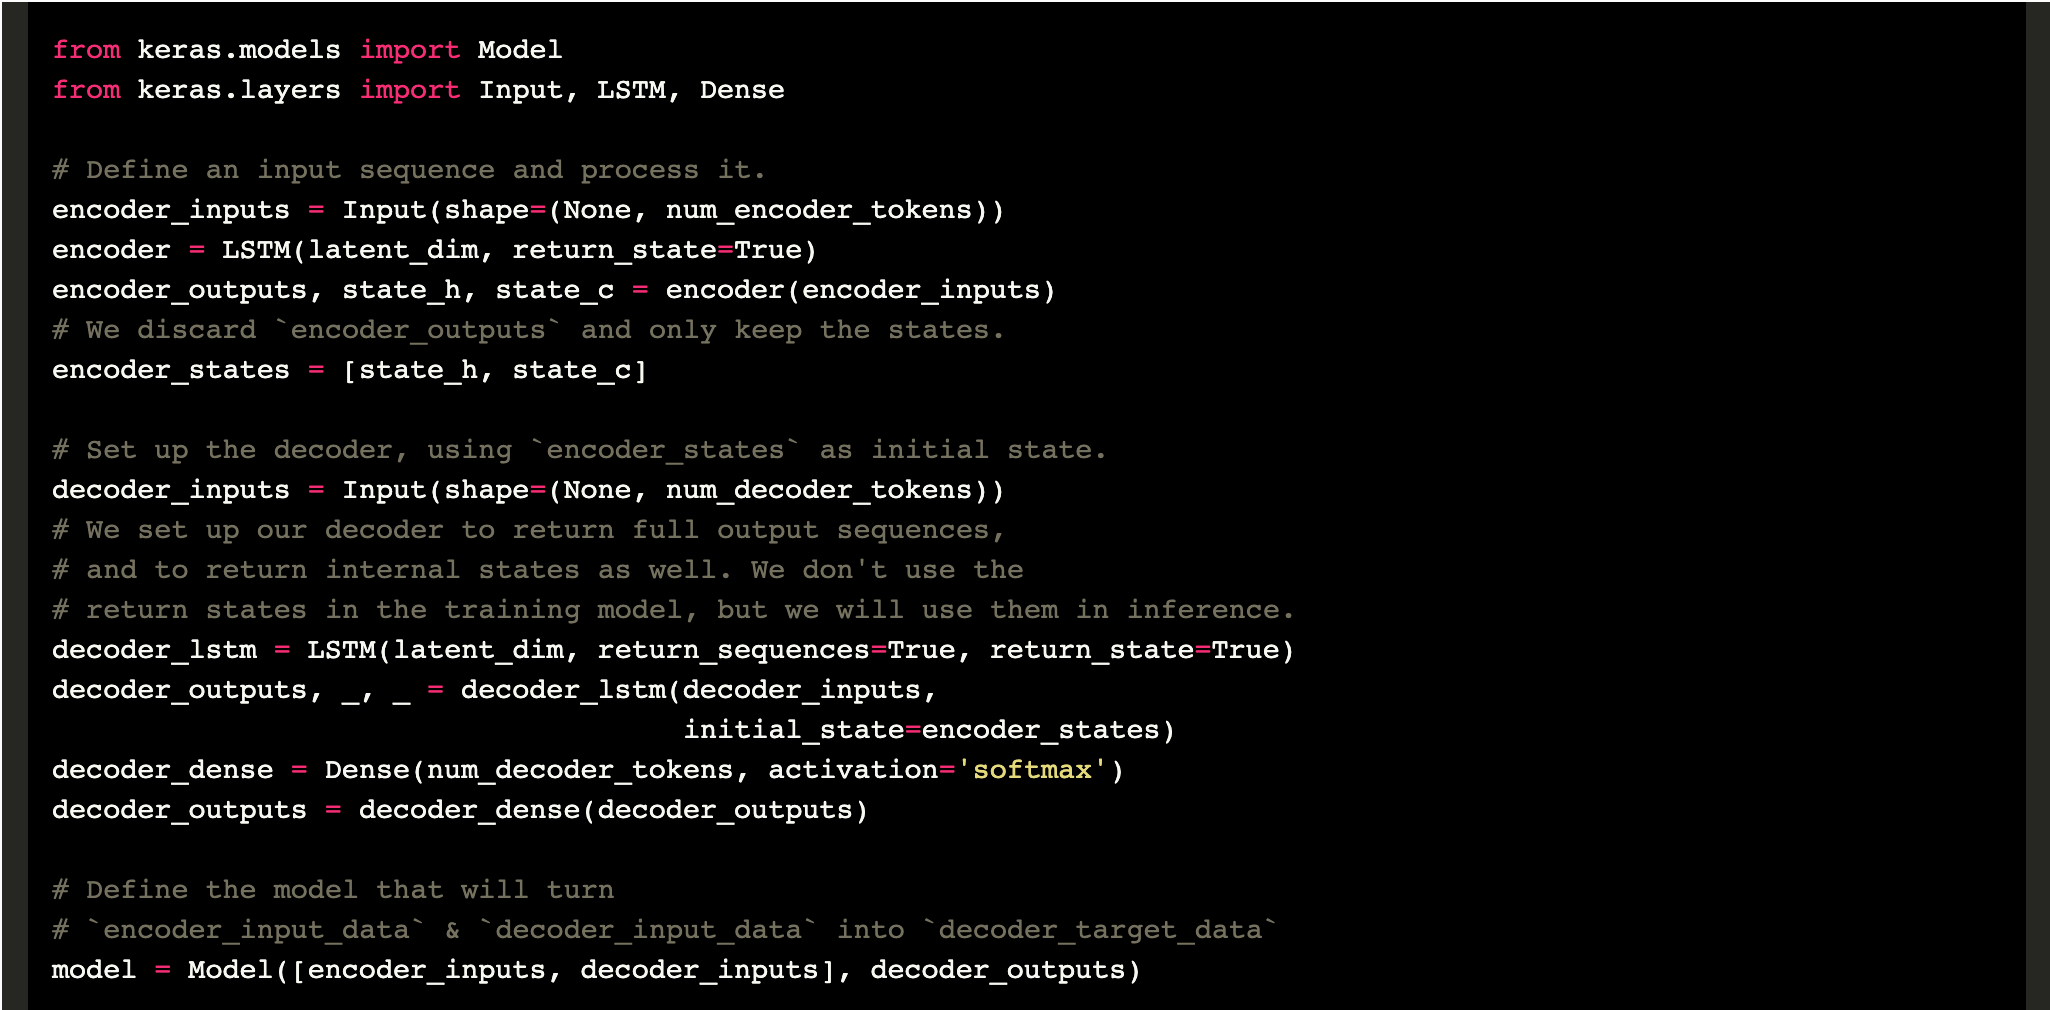
\includegraphics[width=.9\linewidth]{./pictures/rnn_keras.png}
\caption{\label{fig:orgb864b81}
Simple LSTM Implementation}
\end{figure}
\item Attention
\begin{enumerate}
\item For Seq2Seq models.
\begin{enumerate}
\item encoder -> final state.
\begin{enumerate}
\item For each state in decoder, we look at each state in the original encoding and we choose the one that looks most similar
\begin{enumerate}
\item Attention has time complexity of O(l1 * l2) instead of O(l1 + l2) (compared to w/o it)
\end{enumerate}
\end{enumerate}
\end{enumerate}
\end{enumerate}
\item Self Attention
\begin{enumerate}
\item For RNN/LSTM/GRU layers.
\begin{enumerate}
\item For each state in RNN, we look back one state to generate new hidden state

\begin{figure}[ht!]
\centering
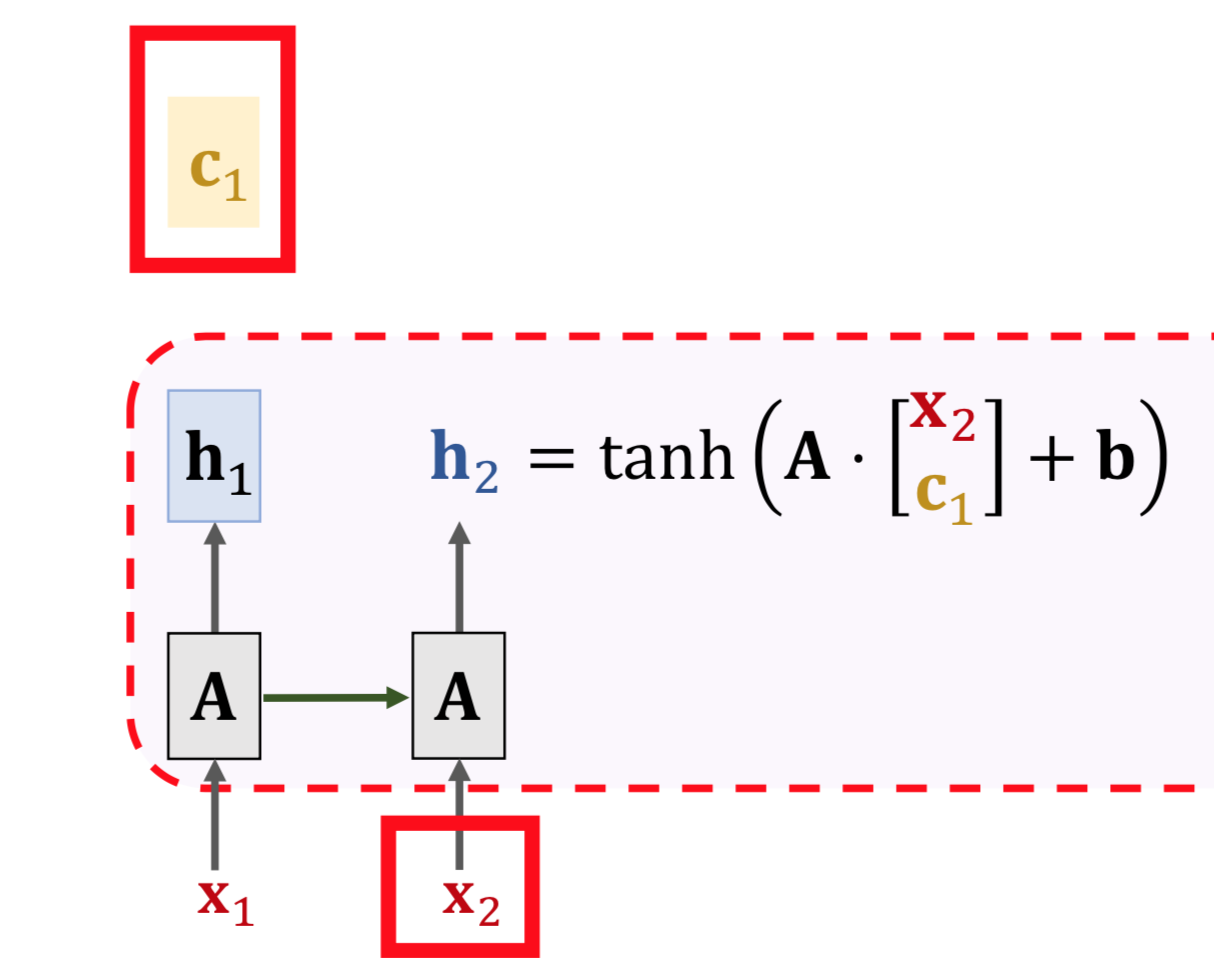
\includegraphics[width=15cm]{./pictures/calc_hidden_state.png}
\caption{\label{fig:org0c482be}
1. Calculating a hidden state}
\end{figure}

---

\item Calculate weights by getting similarity of current hidden state and previous context vector

\begin{figure}[ht!]
\centering
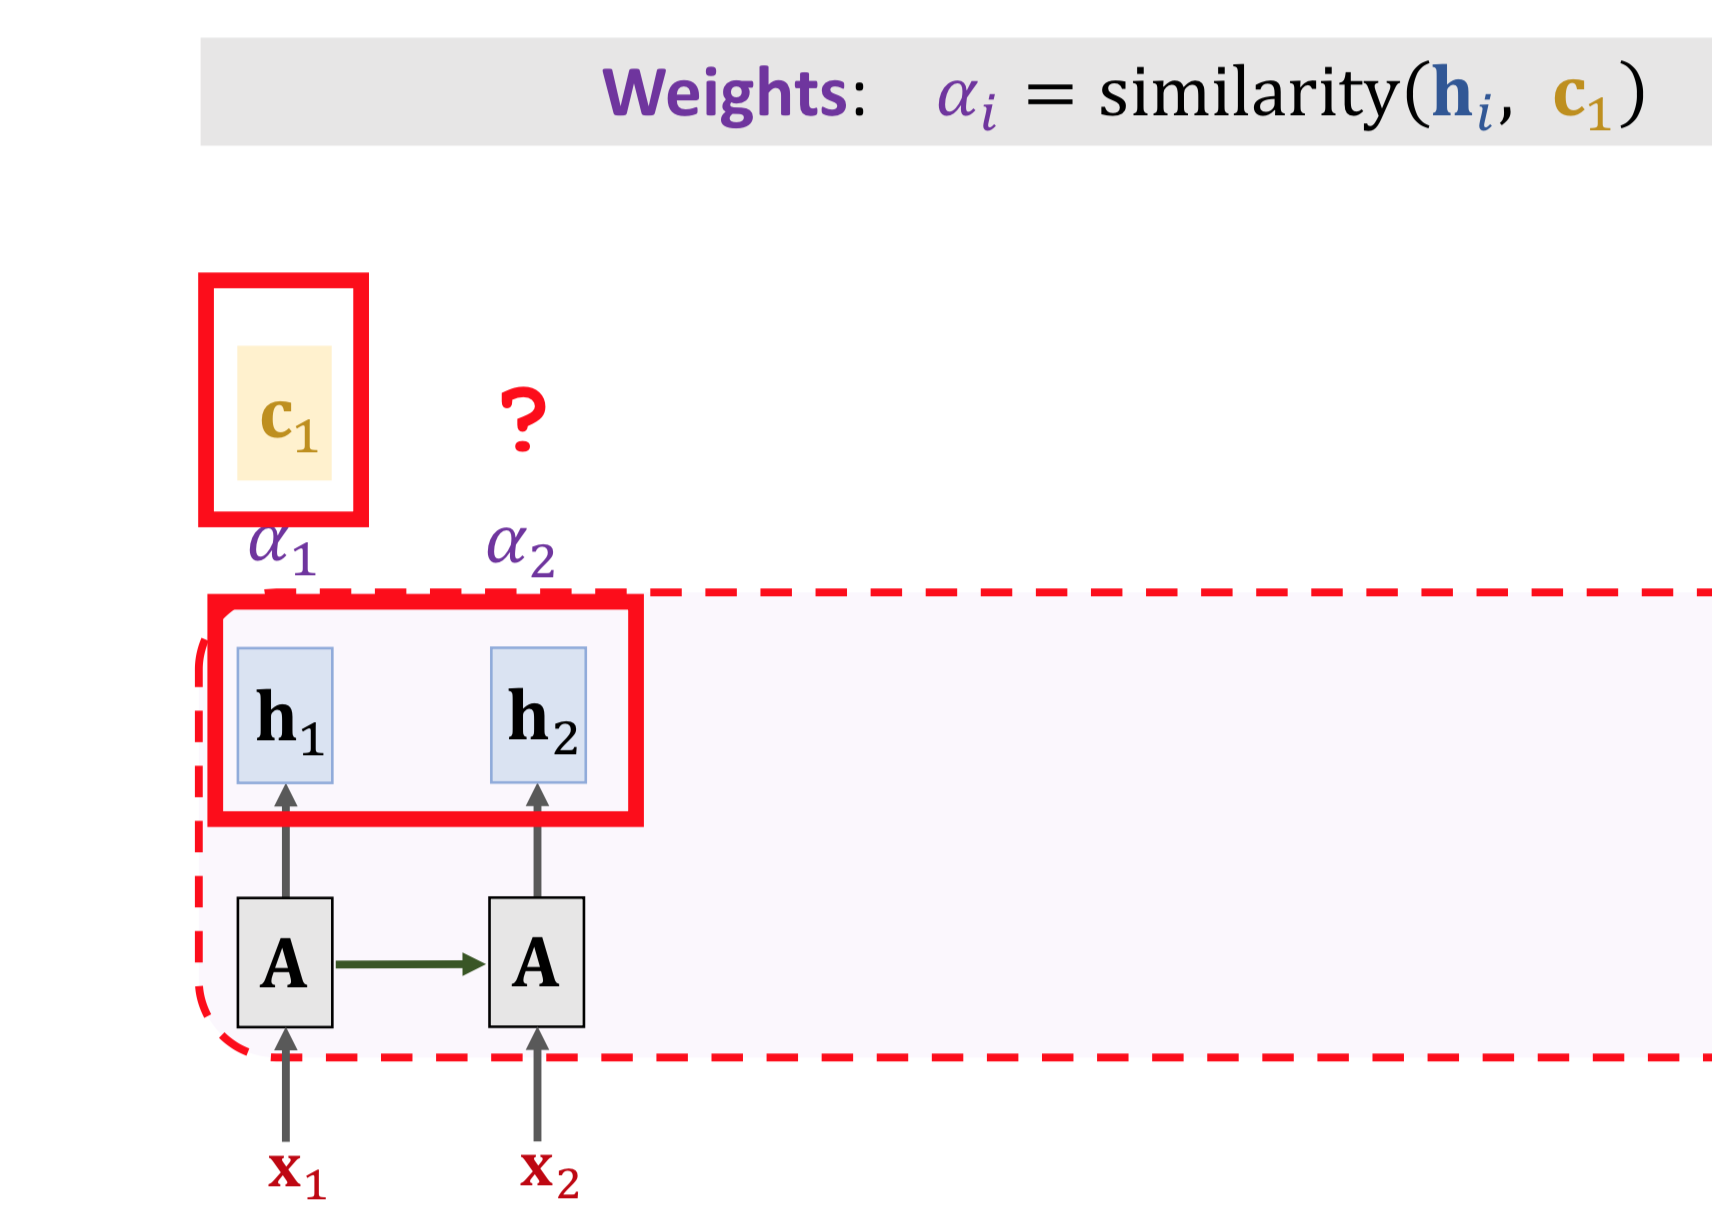
\includegraphics[width=15cm]{./pictures/calc_weights.png}
\caption{\label{fig:org6831be3}
1. Calculating current weight}
\end{figure}

---

\item To Calculate Context vectors, we use use current hidden state and weight and all those from states before

\begin{figure}[ht!]
\centering
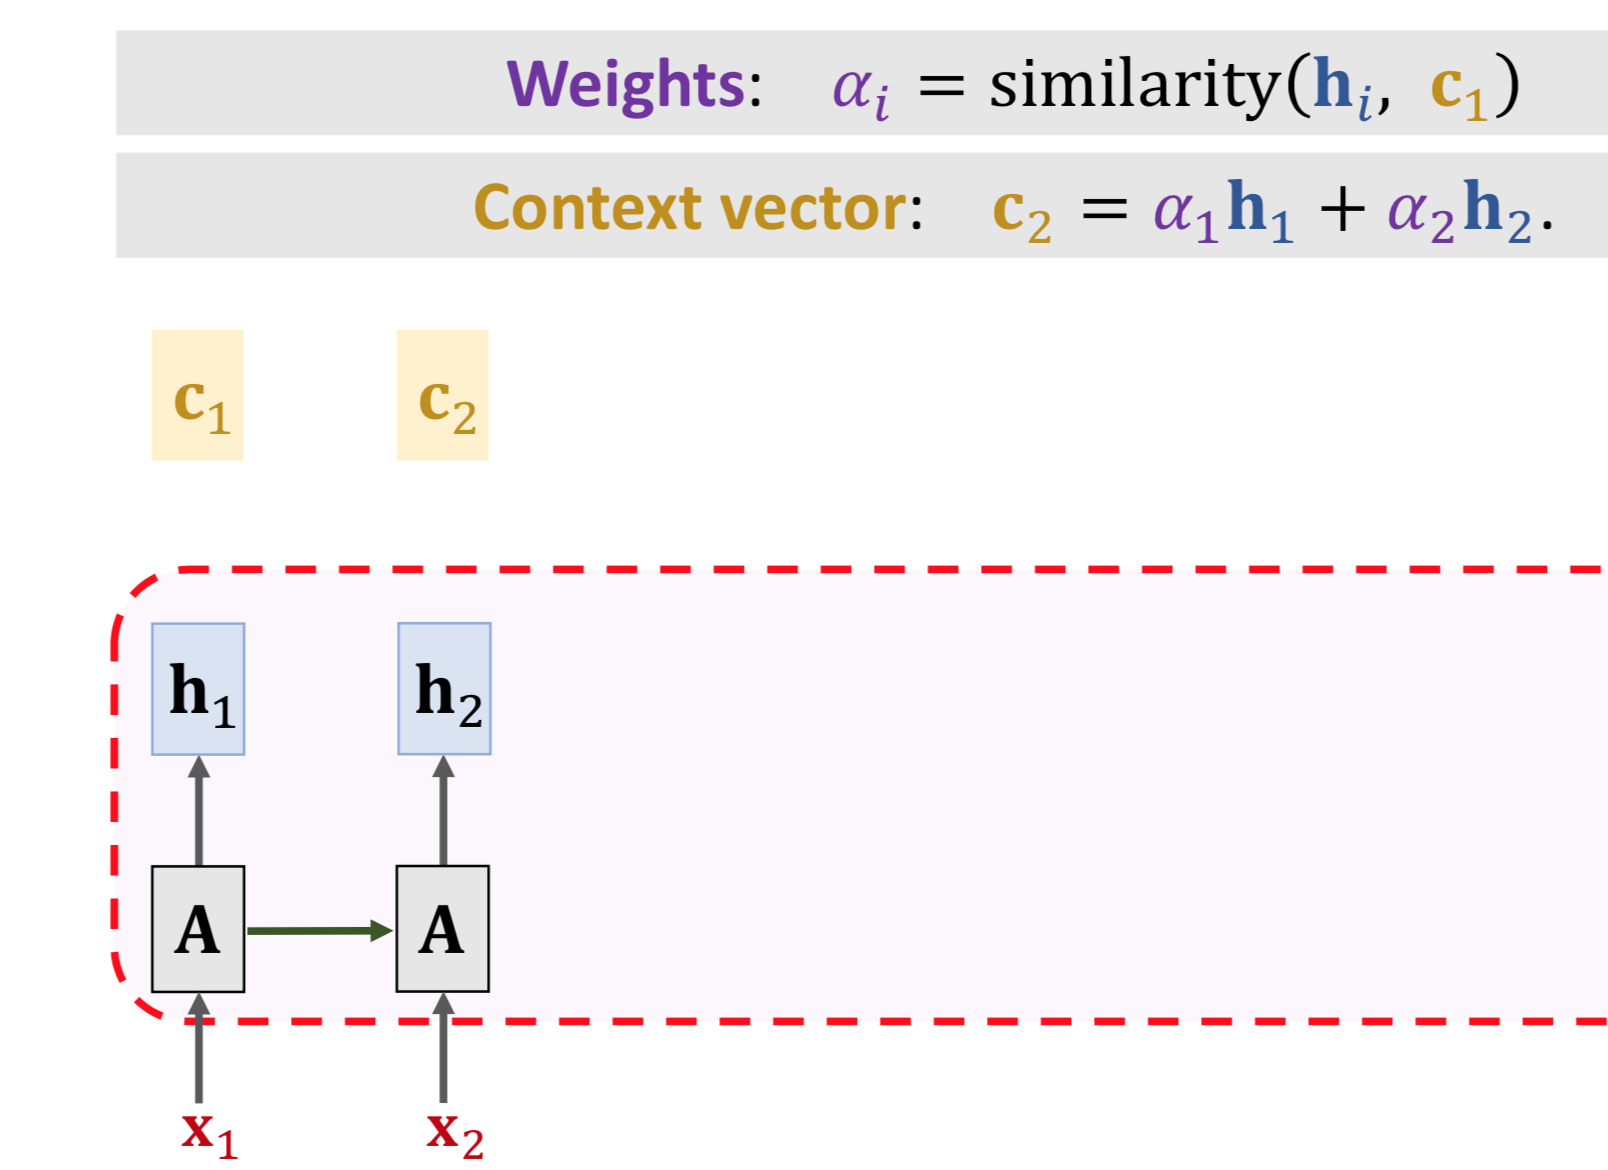
\includegraphics[width=15cm]{./pictures/calc_context_vector.png}
\caption{\label{fig:orgbda3685}
2. Calculating a context vector based on all previous states}
\end{figure}
\end{enumerate}
\end{enumerate}

\item Transformer Model

\begin{enumerate}
\item Is a seq2seq model
\item Uses Multihead attention
\item Not RNN
\item Purely Attention and FC layers
\begin{enumerate}
\item More computation than RNNs
\item Better performance on larger datasets than RNNs

\begin{figure}[ht!]
\centering
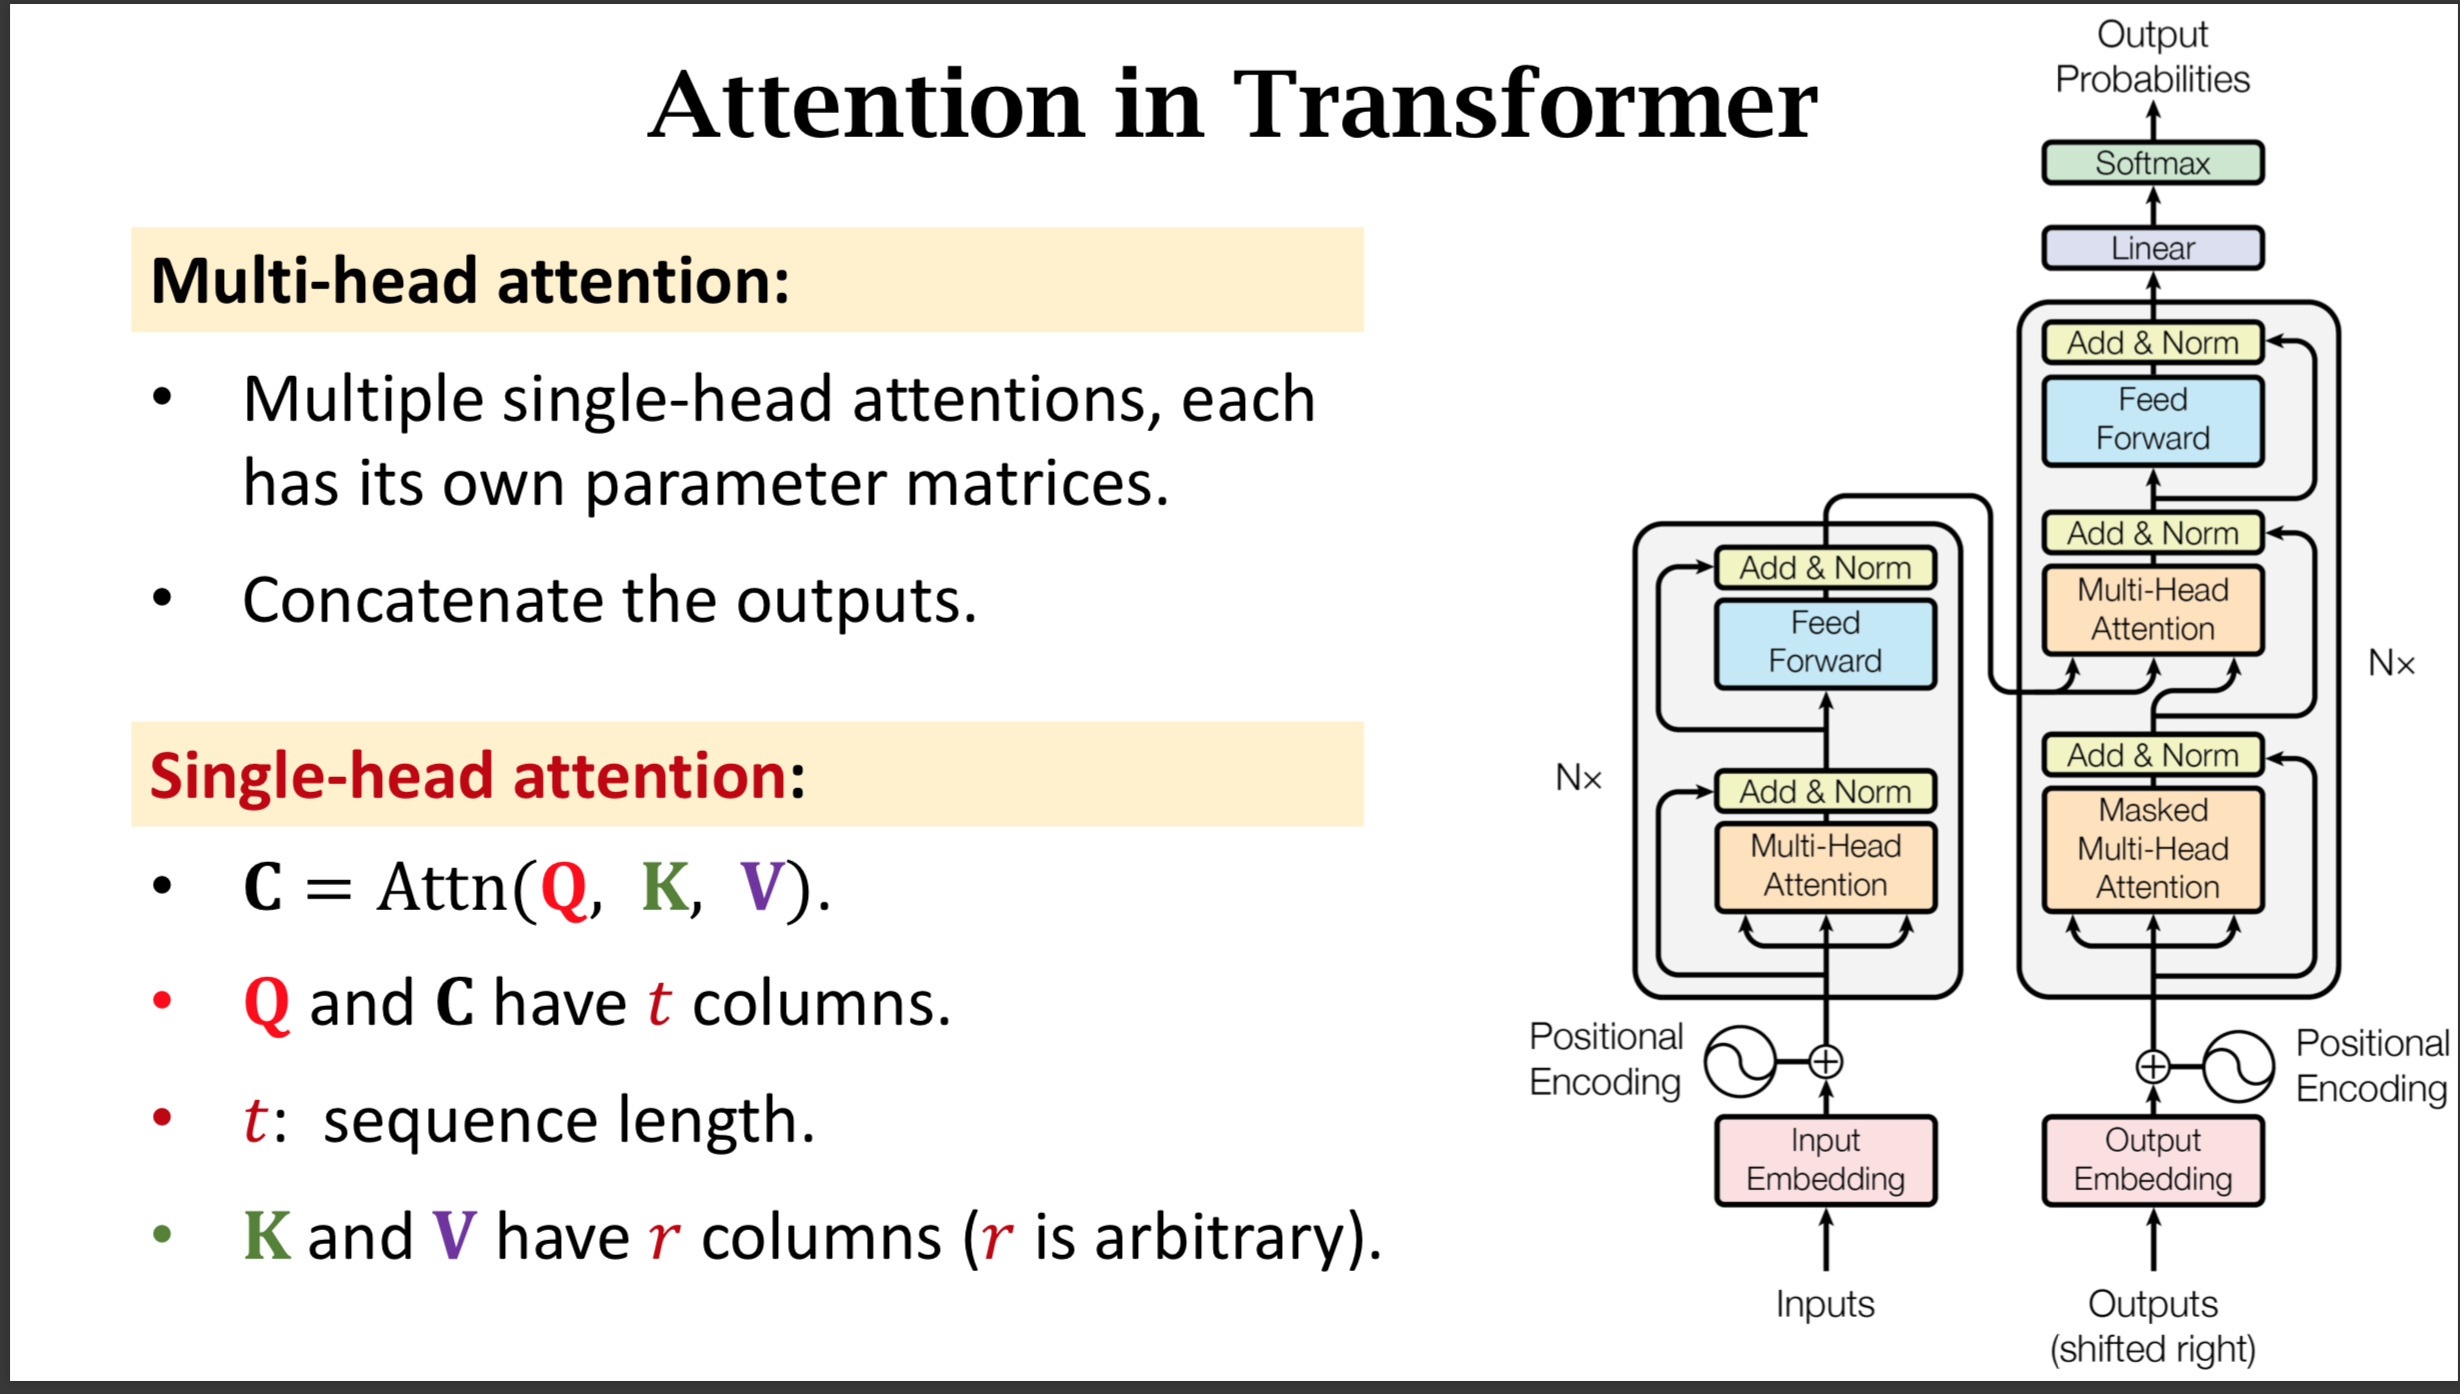
\includegraphics[width=15cm]{./pictures/transformer_params.png}
\caption{\label{fig:org3f297a3}
Transformer Model Attention Parameters}
\end{figure}

\begin{figure}[ht!]
\centering
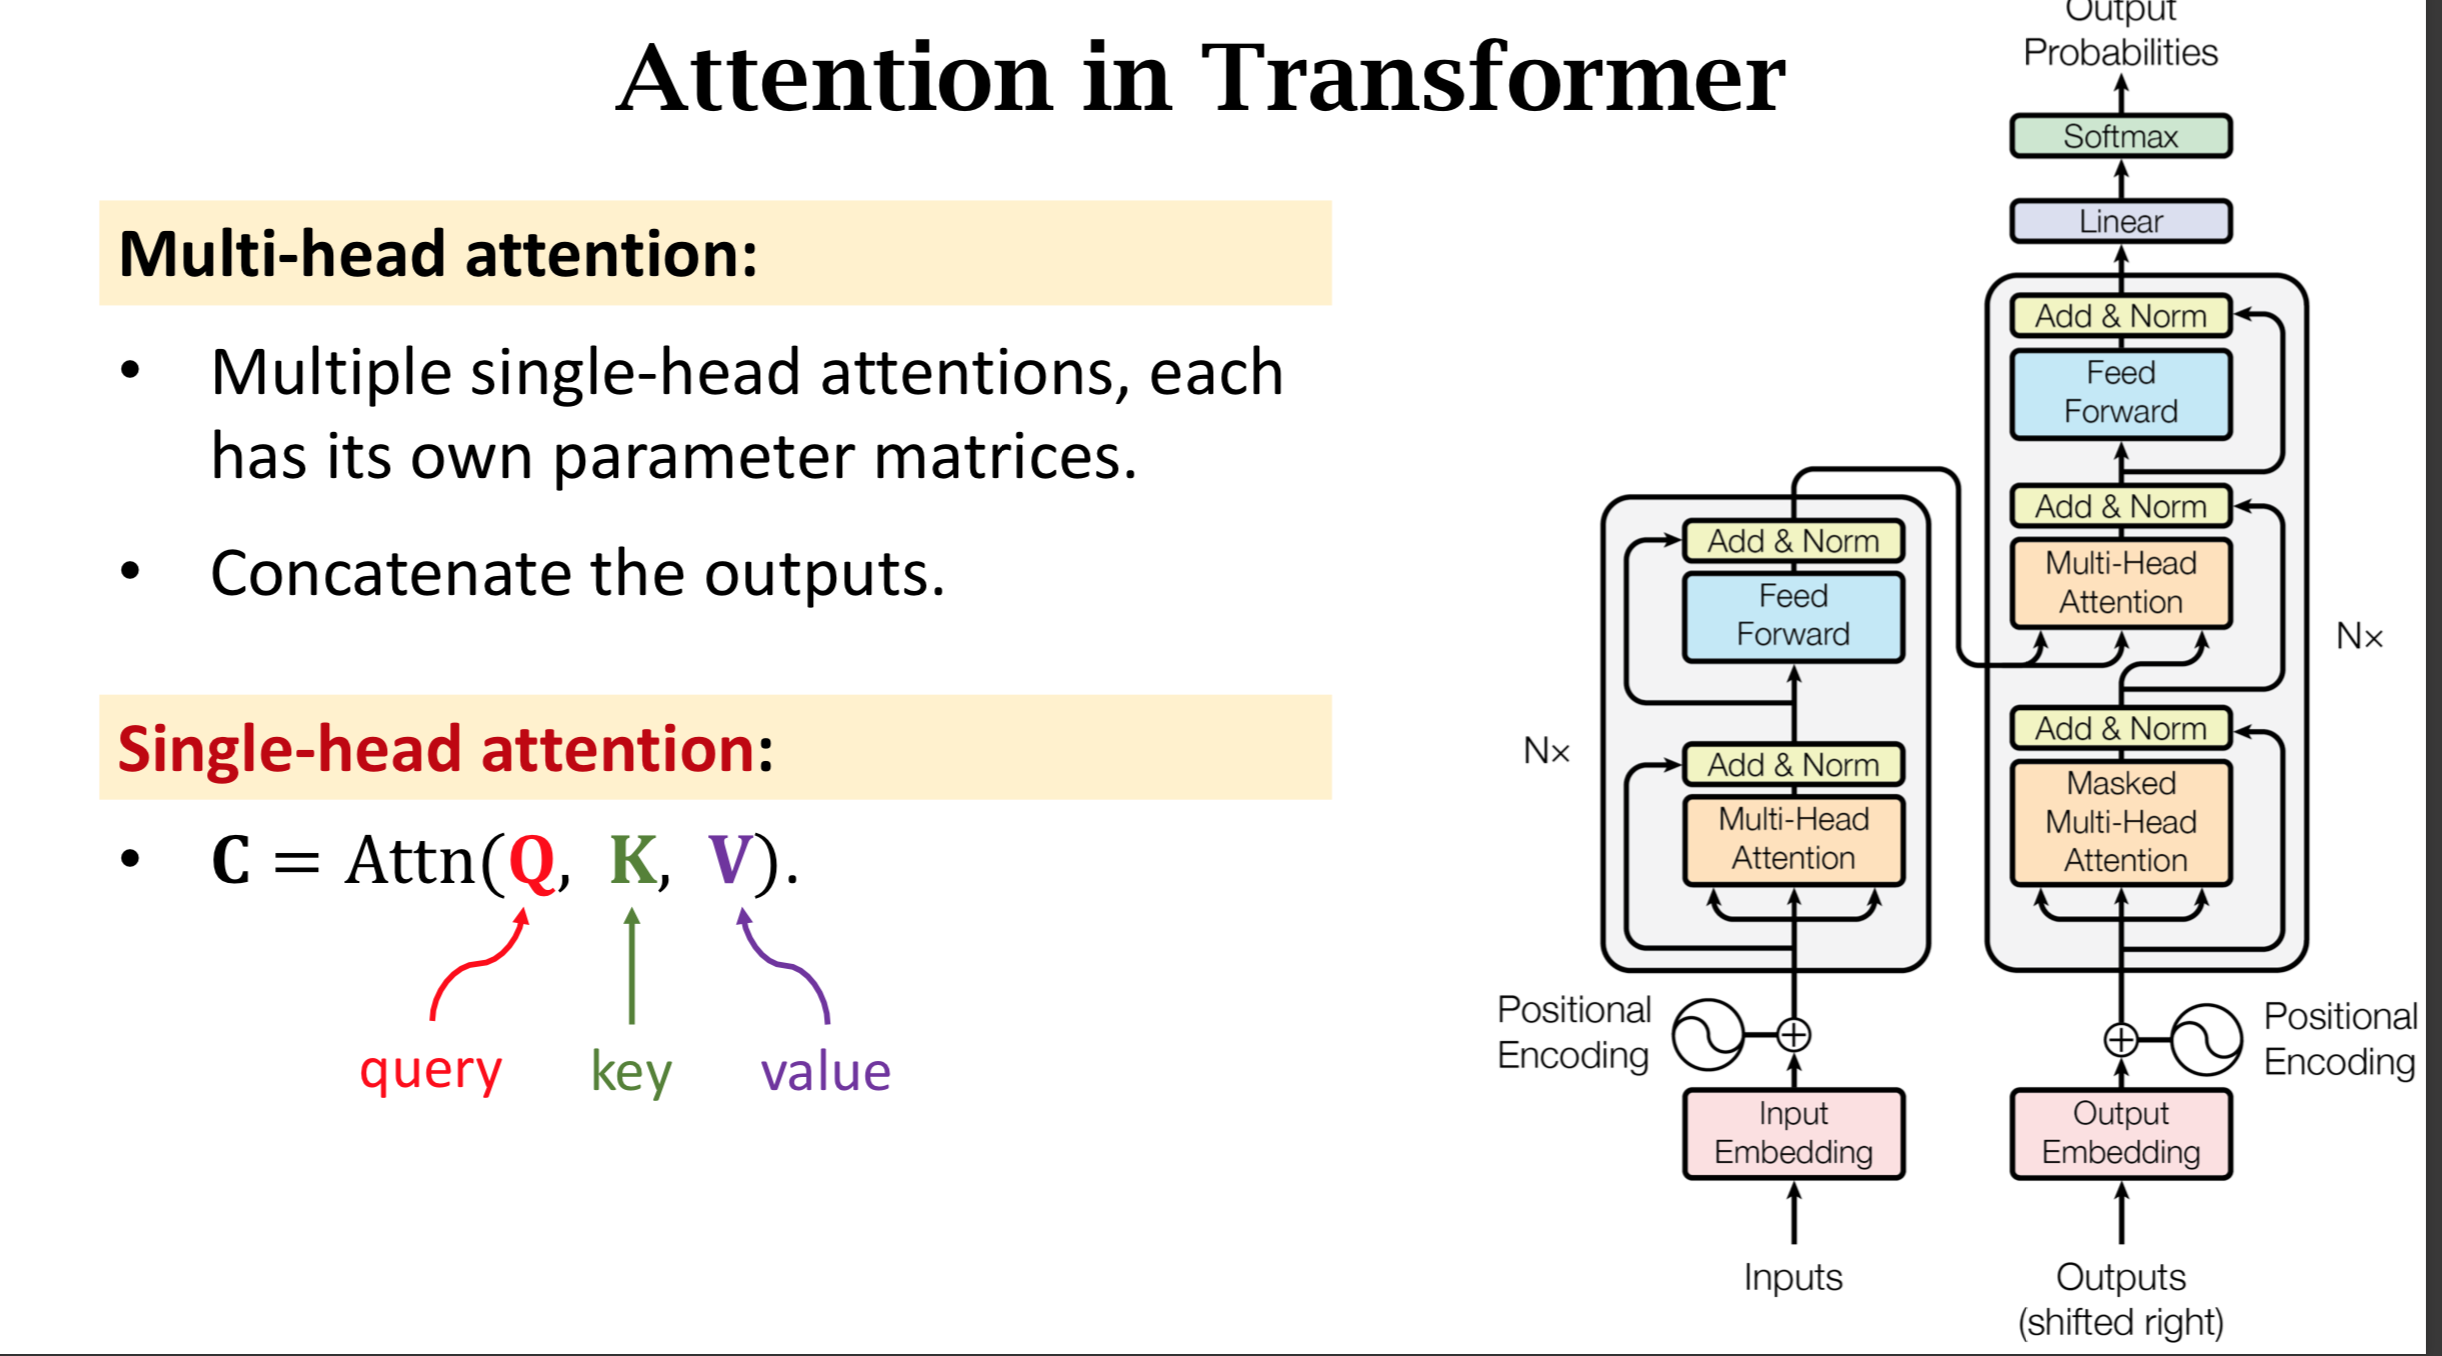
\includegraphics[width=15cm]{./pictures/transformer.png}
\caption{\label{fig:org7f82718}
Transformer Model}
\end{figure}
\end{enumerate}
\end{enumerate}
\end{enumerate}
\section{Number of Trainable parameters}
\label{sec:orgf7a2b1e}

\begin{itemize}
\item Dense: \texttt{output\_size * (input\_size + 1)}
\item Conv2D: \texttt{output\_channels * (input\_channels (kernel\_size + 1))}
\item BatchNormalization: \texttt{4 * input\_channels}
\item RNN: \texttt{output\_shape * (output\_shape + input\_channels) + output\_shape}
\item LSTM: \texttt{4 * RNN}
\end{itemize}



\section{Facial Recognition}
\label{sec:orgcc702f9}

\begin{enumerate}
\item Softmax classifier is bad bc its a Dense Output Layer w/ activation function of Softmax
\begin{enumerate}
\item \# trainable parameters for Dense is \texttt{output\_size * (input\_size + 1)}
\item If \# faces \textasciitilde{}= 10M, and input\_size = 1000, then \# trainable parameters = 10M * 1000 = 10G
\end{enumerate}
\end{enumerate}

\section{Definitions}
\label{sec:org77120d6}

\begin{enumerate}
\item Precision: How many selected items are relevant?
\begin{enumerate}
\item \texttt{relevant items / all items}
\end{enumerate}
\item Recall: How many relevant items are selected?
\begin{enumerate}
\item \texttt{relevant items / all relevant items}
\end{enumerate}
\item Positive Semidefinite
\begin{enumerate}
\item For convex functions, the Hessian Matrix is positive semidefinite everywhere
\end{enumerate}
\end{enumerate}
\end{document}
